\documentclass[11]{beamer}
\usetheme{Warsaw}
\usepackage[utf8]{inputenc}
\usepackage{amsmath}
\usepackage{amsfonts}
\usepackage{amssymb}
\usepackage{color}
\usepackage{siunitx}
%\usepackage[table]{xcolor} 
\usepackage{color, colortbl}

\definecolor{LightCyan}{rgb}{0.88,1,1}
\definecolor{lightgray}{gray}{0.9}
\usepackage{tikz}
\usetikzlibrary{shapes,snakes,arrows,positioning}


% Define box and box title style
\tikzstyle{mybox} = [draw=red, fill=blue!20, very thick,
    rectangle, rounded corners, inner sep=10pt, inner ysep=20pt]
\tikzstyle{fancytitle} =[fill=red, text=white]

\author{Arindam Basu \hspace{5 cm}\newline{arindam@barc.gov.in}}
\title{Accelerator Technology-Vacuum \newline{Vacuum Introduction Part-1}}

%\setbeamercovered{transparent} 
%\setbeamertemplate{navigation symbols}{} 
%\logo{} 
\institute{IADD,BARC} 
%\date{} 
\subject{Accelerator Technology-Vacuum} 
\begin{document}

\begin{frame}
\titlepage
\end{frame}

%\begin{frame}
%\tableofcontents
%\end{frame}





\begin{frame}{Classification of Vacuum}
Vacuum can be classified in three broader categories. These are 
\begin{center}
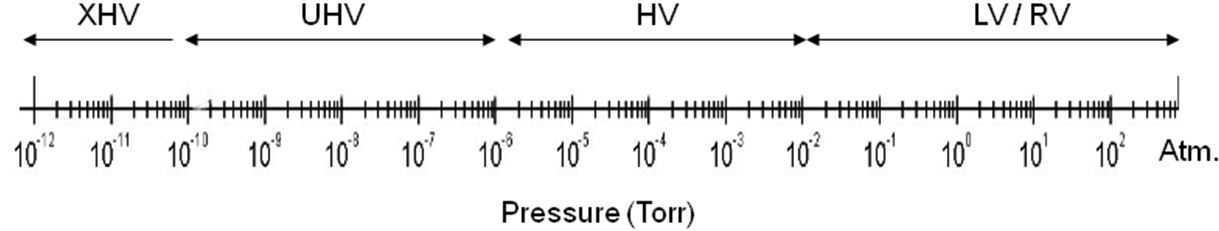
\includegraphics[width=0.5\textwidth]{Vacuum_Scale.png}
\end{center}

\begin{block}{}
	\begin{itemize}
		\item  Rough Vacuum :  759 to $1x 10^{-3}$ Torr
		\item  High Vacuum   :  $1x 10^{-3}$ Torr to $1x 10^{-6}$  Torr
		\item  Ultrahigh Vacuum  :$1x 10^{-6}$  Torr to $1x 10^{-10}$ Torr
		\item  Extra High Vacuum : Less than $1x 10^{-10}$ Torr
	\end{itemize}

\end{block}

\end{frame}





 




\begin{frame}{• Vacuum Establishment}

\begin{exampleblock}

\begin{enumerate}

\item Removal of gas molecules do not happen automatically. To establish vacuum molecules are pumped out of the vacuum system.
\item A vacuum pump is a device which removes gas molecules from the vacuum chamber. 
\item Removal of the gas molecules are done by 
\begin{itemize}
 \item Driving out molecules from the system.
 \item Absorbing molecules in a trap.
 \item Chemically changing the molecules.
\end{itemize}
 
\item Based on these principles different types of vacuum pumps are built.

\end{enumerate}

\end{exampleblock}		


\end{frame}





\begin{frame}{Classification of Vacuum Pumps}
\begin{center}
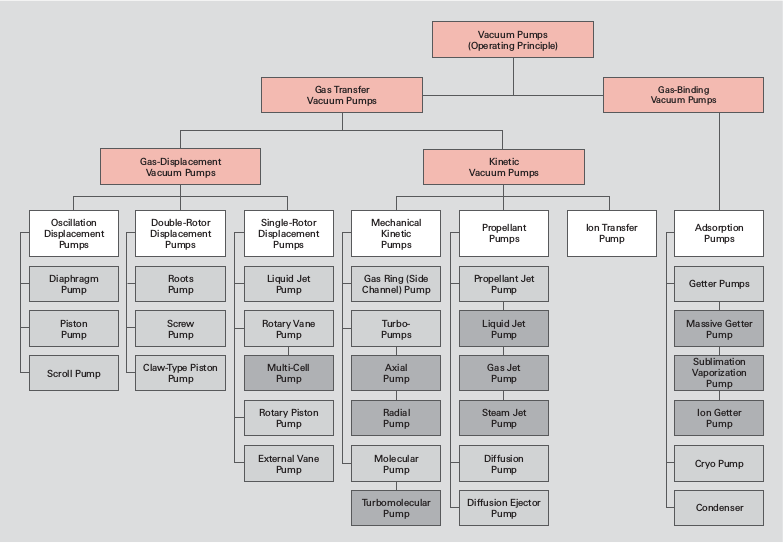
\includegraphics[width=0.9\textwidth]{OverviewOfVacuumPumps.png}
\end{center}
\end{frame}




\begin{frame}{Vacuum Pumps for Various Vacuum Rages}

\begin{enumerate}
\item Pumps for Low vacuum
	\begin{itemize}
	\item Rotary vane pump
    \item    Roots Blowers
     \item   Scroll
      \item  Diaphragm
      \item  Rotary Piston
      \item  Cryo-sorption
     \item   Reciprocating Piston pump
	\end{itemize}
	
\item Pumps for High vacuum
        
        \begin{itemize}
			\item Vapour Diffusion pumps	
    		\item    Turbo Molecular Pump
	    \end{itemize}
	
\item Pumps for Ultra High vacuum
        
        \begin{itemize}
			\item Turbomolecular pump
      		\item 	 Sputter Ion Pump
       		\item 		Cryogenic Pump
       		\item 		Titanium Sublimation pump
       		\item 		NEG Pumps
    		   
	    \end{itemize}


\end{enumerate}


\end{frame}





\begin{frame}{Types of }

\end{frame}






\begin{frame}

\end{frame}




\begin{frame}

\end{frame}






\begin{frame}

\end{frame}






\begin{frame}

\end{frame}





%\begin{frame}
%\begin{thebibliography}{10}
%\bibitem{Goldbach1742}[Goldbach, 1742]
%Christian Goldbach.
%\newblock A problem we should try to solve \break before the ISPN ’43 deadline,
%\newblock \emph{Letter to Leonhard Euler}, 1742.
%\end{thebibliography}

%\begin{block}{Open Questions}
%Is every even number the sum of two primes?
%\cite{Goldbach1742}
%\end{block}
%\end{frame}









\end{document}